\section{Product}

\subsection{FPGA}
The responsibilities of the FPGA consist of three major parts: PWM to control the speed of the two engine mounted on the PanTilt platform; An encoder which data is used together with a timestamp to calculate speed and see the direction the engine is turning; and SPI communication receive values for the PWM and send data back the the ARM board so that the necessary calculations can be made.

Each of these three have been created in its own separate component, and is encapsled in a main component called the Motor Controller.


\subsubsection{Motor Controller}

The FPGA have been designed in such a way that each engine has its own Motor controller.

...

Furthermore a reset button have been implemented as a safety precaution, so it is possible to stop the engines manually if something unintended were to happen. The button is setup in such a way that when it is pressed the Timestamp, PWM and Encoder value will be cleared ensuring that the engines stop. The reset button is also connection to the ARM board by a reset line, so the ARM board can turn the engines back to start position.

SW(0) and SW(1) have been connected to the H-Bridge enable, so by turning one of them off the signal to the engine will be disabled. This is useful for both testing and as another safety precaution.

\paragraph{SPI Controller}\mbox{}\\

\textbf{PISO}\\
The Parallel In Serial Out (PISO) component is used to send data from the FPGA to the ARM board. It functions like a shift register that takes parallel input from the encoder and shift it out serial.

\begin{figure}[h]
	\centering
	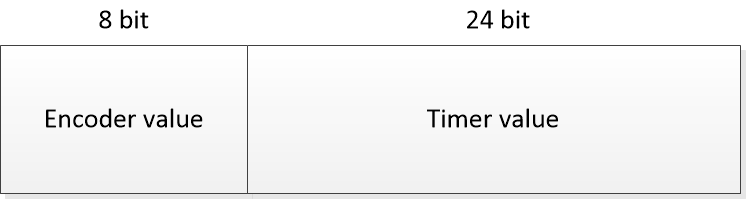
\includegraphics[scale=2]{PISO_Format}
	\caption{Frame format for the PISO}
	\label{PISO_Format}
\end{figure}

billede \ref{PISO_Format} har labelet abelars

\textbf{SIPO}\\
The Serial In Parallel Out (SIPO) component is used to receive data from the ARM board to the FPGA. It functions like a shift register that receives a serial input from MOSI and outputs it Parallel to the PWM. The SIPO is 9-bit wide, 8 of the bits is the PWM value and the MSB is 

\begin{figure}[h]
	\centering
	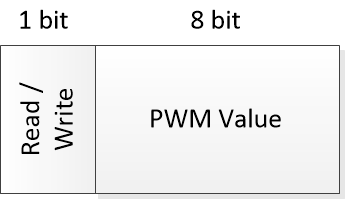
\includegraphics[scale=2]{SIPO_Format}
	\caption{Frame format for the SIPO}
	\label{SIPO_Format}
\end{figure}

billede \ref{SIPO_Format} har labelet abelars


\textbf{Encoder Controller}

\textbf{PWM Controller}